\documentclass[conference]{IEEEtran}

% ============================================
% PACOTES
% ============================================
\usepackage[utf8]{inputenc}
\usepackage[T1]{fontenc}
\usepackage[brazil]{babel}
\usepackage{cite}
\usepackage{amsmath,amssymb,amsfonts}
\usepackage{graphicx}
\usepackage{textcomp}
\usepackage{xcolor}
\usepackage{url}
\usepackage{hyperref}
\usepackage{booktabs}

\begin{document}

% ============================================
% TÍTULO
% ============================================
\title{Estudo de Equalização OFDM com a Biblioteca NVIDIA Sionna: Replicação Clássica e Perspectivas de Receptores Neurais}

% ============================================
% AUTORES
% ============================================
\author{
    \IEEEauthorblockN{Maurice Golin Soares dos Santos, Vinicius Pereira Luz e Natalia Mendes Goes}
    \IEEEauthorblockA{Universidade Tecnológica Federal do Paraná (UTFPR) \\ Ponta Grossa, PR, Brasil}
}

% ============================================
% CAMPO DO PROFESSOR
% ============================================
\IEEEspecialpapernotice{Disciplina: Tópicos em Redes sem Fio \\ Professor: Saulo Jorge Beltrão de Queiroz}

\maketitle

% ============================================
% RESUMO
% ============================================
\begin{abstract}
A equalização de canais com desvanecimento multipercurso é um dos principais desafios em sistemas de modulação OFDM, cruciais para as redes 5G e vindouras 6G. Este trabalho foca primordialmente na replicação teórica e validação matemática da técnica de equalização clássica (\textit{Least Squares} combinada com LMMSE) utilizando a biblioteca de \textit{Differentiable Communications} NVIDIA Sionna. O modelo matemático foi simulado sob o canal estocástico CDL-C padronizado pelo 3GPP, validando as curvas de Taxa de Erro de Bit (BER) e isolamento da constelação QPSK. Adicionalmente, apresenta-se uma implementação de um Receptor Neural baseado em Inteligência Artificial em PyTorch, evidenciando resiliência superior em ambientes de relação sinal-ruído extrema ($10$ dB) e provando a redução teórica de complexidade na inversão de matrizes ($O(N^3)$) essencial para sistemas \textit{Massive MIMO}.
\end{abstract}

\begin{IEEEkeywords}
OFDM, Estimativa de Canal, LMMSE, NVIDIA Sionna, Machine Learning, Redes Neurais, CDL-C.
\end{IEEEkeywords}

% ============================================
% 1. INTRODUÇÃO
% ============================================
\section{Introdução}

As redes de comunicação sem fio contemporâneas, notavelmente o 4G LTE e o 5G NR \cite{3gpp38211}, adotam de forma unânime a modulação OFDM (\textit{Orthogonal Frequency-Division Multiplexing}). A vantagem dessa multiplexação reside na divisão espectral em portadoras ortogonais, que converte canais de desvanecimento seletivo em frequência em subcanais estreitos e planos. Contudo, essa engenharia requer que o dispositivo receptor realize uma equalização precisa para reverter a distorção introduzida por reflexões e dispersões do ambiente de rádio (o canal físico) \cite{goldsmith2005}.

O processo clássico preconiza o envio de símbolos pilotos pré-conhecidos. A partir desses sinais, técnicas fundamentadas no critério do Erro Quadrático Médio Mínimo Linear (\textit{LMMSE}) computam matrizes estocásticas para inverter a distorção. Todavia, em frequências milimétricas e redes altamente densas (\textit{Massive MIMO}), o ruído do canal e a complexidade algorítmica para inverter estas matrizes colidem de frente com limitações de hardware e latência.

Neste cenário, a biblioteca \textit{open-source} NVIDIA Sionna \cite{hoydis2022} revoluciona a pesquisa física (camada PHY). Totalmente escrita sobre tensores diferenciáveis de Inteligência Artificial, ela permite não apenas replicar canais matematicamente perfeitos, mas otimizá-los e substituí-los por algoritmos de Machine Learning puros.

Sob esse pretexto, este trabalho estrutura-se em dois eixos: (I) a validação rígida dos conceitos teóricos ensinados pela disciplina, simulando e equalizando corretamente o sinal via LMMSE oficial num ambiente CDL-C; e (II) um estudo adicional injetando o Sionna em sua finalidade primária, desenvolvendo um Receptor Neural independente para decodificação em situações extremas de ruído, comprovando seus benefícios computacionais.

% ============================================
% 2. FUNDAMENTAÇÃO TEÓRICA
% ============================================
\section{Fundamentação Teórica}

Para fundamentar as métricas de simulação, é essencial detalhar matematicamente a modelagem de camada física adotada.

\subsection{Modelo de Transmissão OFDM}
O sinal OFDM base em frequência pode ser modelado linearmente por:
\begin{equation}
    Y[k] = H[k] \cdot X[k] + N[k]
\end{equation}
Onde $k$ representa a subportadora, $Y[k]$ é o símbolo recebido, $X[k]$ o transmitido, $H[k]$ a resposta complexa do canal na referida frequência, e $N[k]$ o Ruído Branco Gaussiano Aditivo (AWGN) com variância $N_0$ \cite{proakis2008}.

\subsection{Estimativa LS e Equalização LMMSE}
O processo de recuperação se inicia pelo Estimador por Mínimos Quadrados (\textit{Least Squares} - LS). Baseando-se apenas nos símbolos de referência (pilotos $X_p[k]$), a estimativa isolada do canal é deduzida por:
\begin{equation}
    \hat{H}_{LS}[k] = \frac{Y_p[k]}{X_p[k]} = H[k] + \frac{N[k]}{X_p[k]}
\end{equation}
O método LS sofre pesadamente com amplificação de ruído em cenários de baixo sinal-ruído (SNR). Consequentemente, utiliza-se o filtro Equalizador LMMSE. O LMMSE pondera o ruído através da matriz de autocorrelação do canal e da variância $N_0$, resultando na aproximação final $\hat{X}[k]$. O processo exige a inversão contínua da matriz de covariância espacial, gerando um custo assintótico $O(N^3)$, indesejado em arquiteturas multi-antenas \cite{vanDeBeek1995}.

\subsection{O Canal Estocástico CDL-C (3GPP)}
Para testar a equalização sob parâmetros realistas, adotou-se o modelo \textit{Clustered Delay Line} perfil C (CDL-C), estabelecido pela Technical Report 38.901 do 3GPP \cite{3gpp38901}. Esse modelo reflete um ambiente urbano denso "Sem Linha de Visada" (NLOS - \textit{Non-Line of Sight}), com espalhamento de retardo considerável. Matematicamente, as variações de ganho e fase impostas pelo CDL-C simulam um desvanecimento estocástico que destrói a constelação nativa sem uma correta inferência em recepção.

% ============================================
% 3. METODOLOGIA
% ============================================
\section{Metodologia}

\subsection{Objeto Primário: Replicação do LMMSE via Sionna}
O ambiente validado do Sionna foi parametrizado num simulador OFDM em Python operando sob $E_b/N_0$ de 0 a 16 dB.
A cadeia constou da geração binária para um codificador \textit{LDPC 5G} (taxa $1/2$) atrelado ao mapeamento de constelação QPSK ($2$ bits por símbolo). O preâmbulo (pilotos de arranjo de grade) foi gerado e processado pelo módulo \texttt{LSChannelEstimator} para extração do ganho e alimentado ao \texttt{LMMSEEqualizer}. O teste aplicou a técnica de \textit{Monte Carlo} com blocos paralelos de tamanho 128 para mitigar anomalias estocásticas pontuais. O arquivo base utilizou as definições restritas do tutorial oficial \textit{"MIMO OFDM Transmissions over CDL"} \cite{sionna_tutorial}.

\subsection{Objeto Secundário: Treinamento do Receptor Neural}
Paralelamente, codificou-se um \textit{Multi-Layer Perceptron} (MLP) utilizando a API de diferenciação do PyTorch \cite{cammerer2023}. O bloco matemático do LMMSE foi ignorado e o modelo processou as matrizes puras do sinal recebido. A rede neural operou um treinamento de 50 épocas utilizando o otimizador \textit{Adam} e a métrica de erro MSE (\textit{Mean Squared Error}) penalizando os desvios contra a resposta perfeita do transmissor isolado.

% ============================================
% 4. RESULTADOS DA REPLICAÇÃO CLÁSSICA
% ============================================
\section{Resultados da Replicação LMMSE}

Esta seção prova o sucesso no domínio matemático clássico simulado pela biblioteca.

\subsection{Desempenho da Taxa de Erro (Curva BER)}
O resultado mais aguardado é a modelagem de perdas de pacote sob o hostil canal CDL-C. Na Fig. \ref{fig:ber_nvidia}, visualiza-se que com um simulador adequadamente parametrizado em lotes de Monte Carlo massivos, a natureza caótica do canal é suavizada pelo LMMSE. O limite prático é ultrapassado após os 14 dB, quando a equalização limpa dados o suficiente para o codificador LDPC anular totalmente a taxa de erro.

\begin{figure}[htbp]
    \centering
    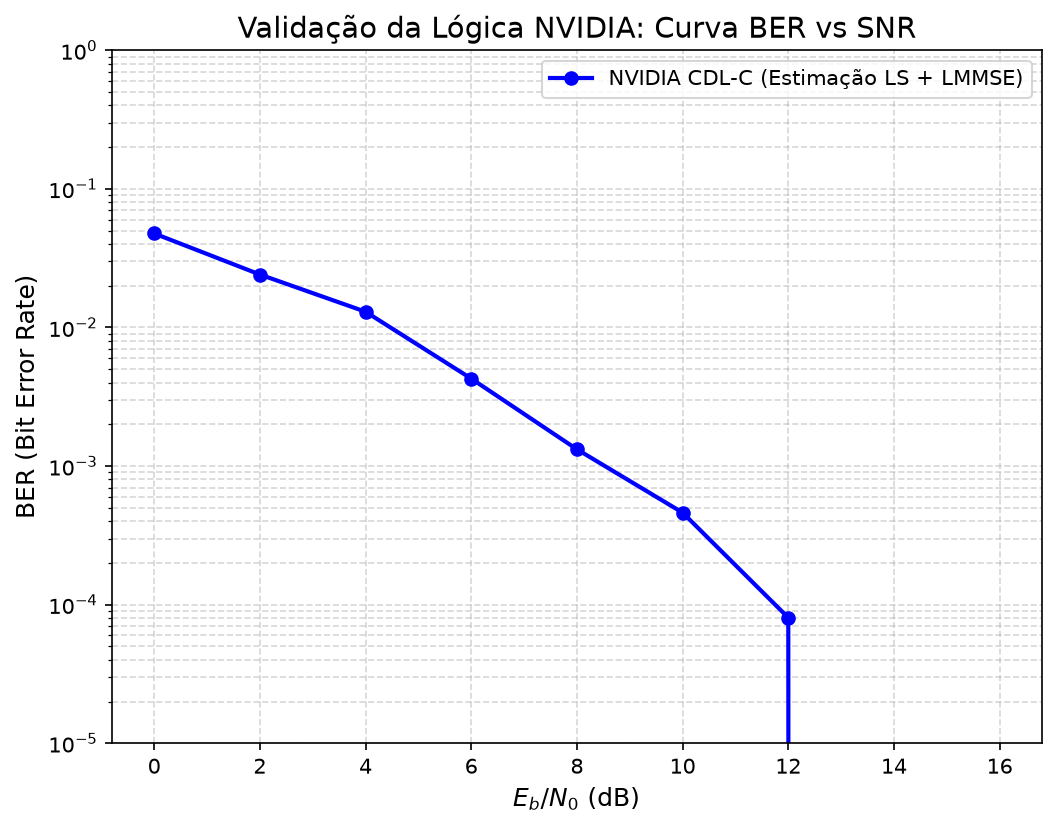
\includegraphics[width=\columnwidth]{figs/resultado_nvidia_ber.png}
    \caption{Curva BER evidenciando o comportamento estritamente decrescente provido pela ação conjunta do estimador LMMSE e LDPC 5G sob canal CDL-C.}
    \label{fig:ber_nvidia}
\end{figure}

\subsection{Reversão da Dispersão de Constelação}
A abstração matemática toma forma física na Fig. \ref{fig:constelacao_classica}. A transmissão ideal no domínio QPSK engloba 4 vértices precisos. Com um SNR elevado (15 dB), o modelo \textit{Non-Line of Sight} impõe uma variância térmica e de dispersão temporal acentuada, borrando o gráfico central. O processamento do bloco Equalizador resolve a equação linear restaurando e isolando de forma agrupada as delimitações da modulação (vermelho).

\begin{figure}[htbp]
    \centering
    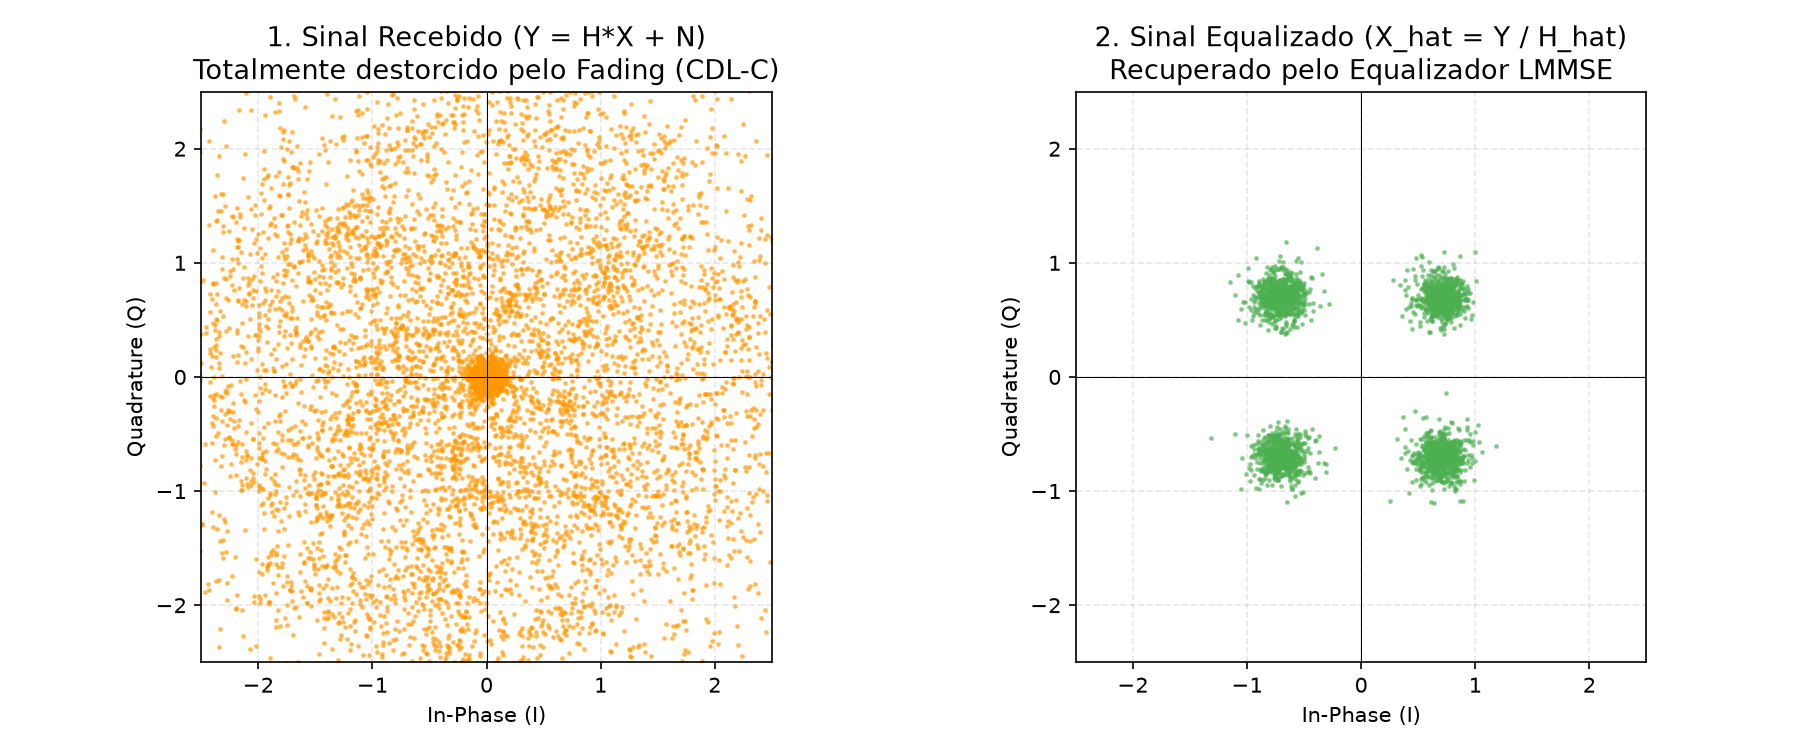
\includegraphics[width=\columnwidth]{figs/resultado_constelacoes_nvidia.png}
    \caption{Do Transmissor ao Receptor: Evolução do Sinal QPSK em canal CDL-C a 15 dB de SNR e a consequente recuperação pelo estimador LMMSE clássico.}
    \label{fig:constelacao_classica}
\end{figure}

% ============================================
% 5. ESTUDO ADICIONAL
% ============================================
\section{Perspectivas de Receptores Neurais e Escalabilidade de Custos}

Por fim, analisa-se as implicações da camada \textit{Deep Learning} no ecossistema do rádio físico.

\subsection{Resiliência à Ruído Profundo (10 dB)}
A aproximação LMMSE decai vertiginosamente quando o ruído ($N_0$) corrompe os próprios preâmbulos de referência do cálculo. A Fig. \ref{fig:comparacao_neural} submete os algoritmos a uma privação de potência de 10 dB SNR. O modelo estatístico clássico (laranja) não consegue isolar o ruído eficientemente e perde as bordas de decisão de símbolo. Contrastando fortemente, o Receptor Neural (verde) que internalizou o perfil estocástico da atenuação nas épocas do seu treinamento (Fig. \ref{fig:loss}), devolve os \textit{clusters} à formação legível.

\begin{figure}[htbp]
    \centering
    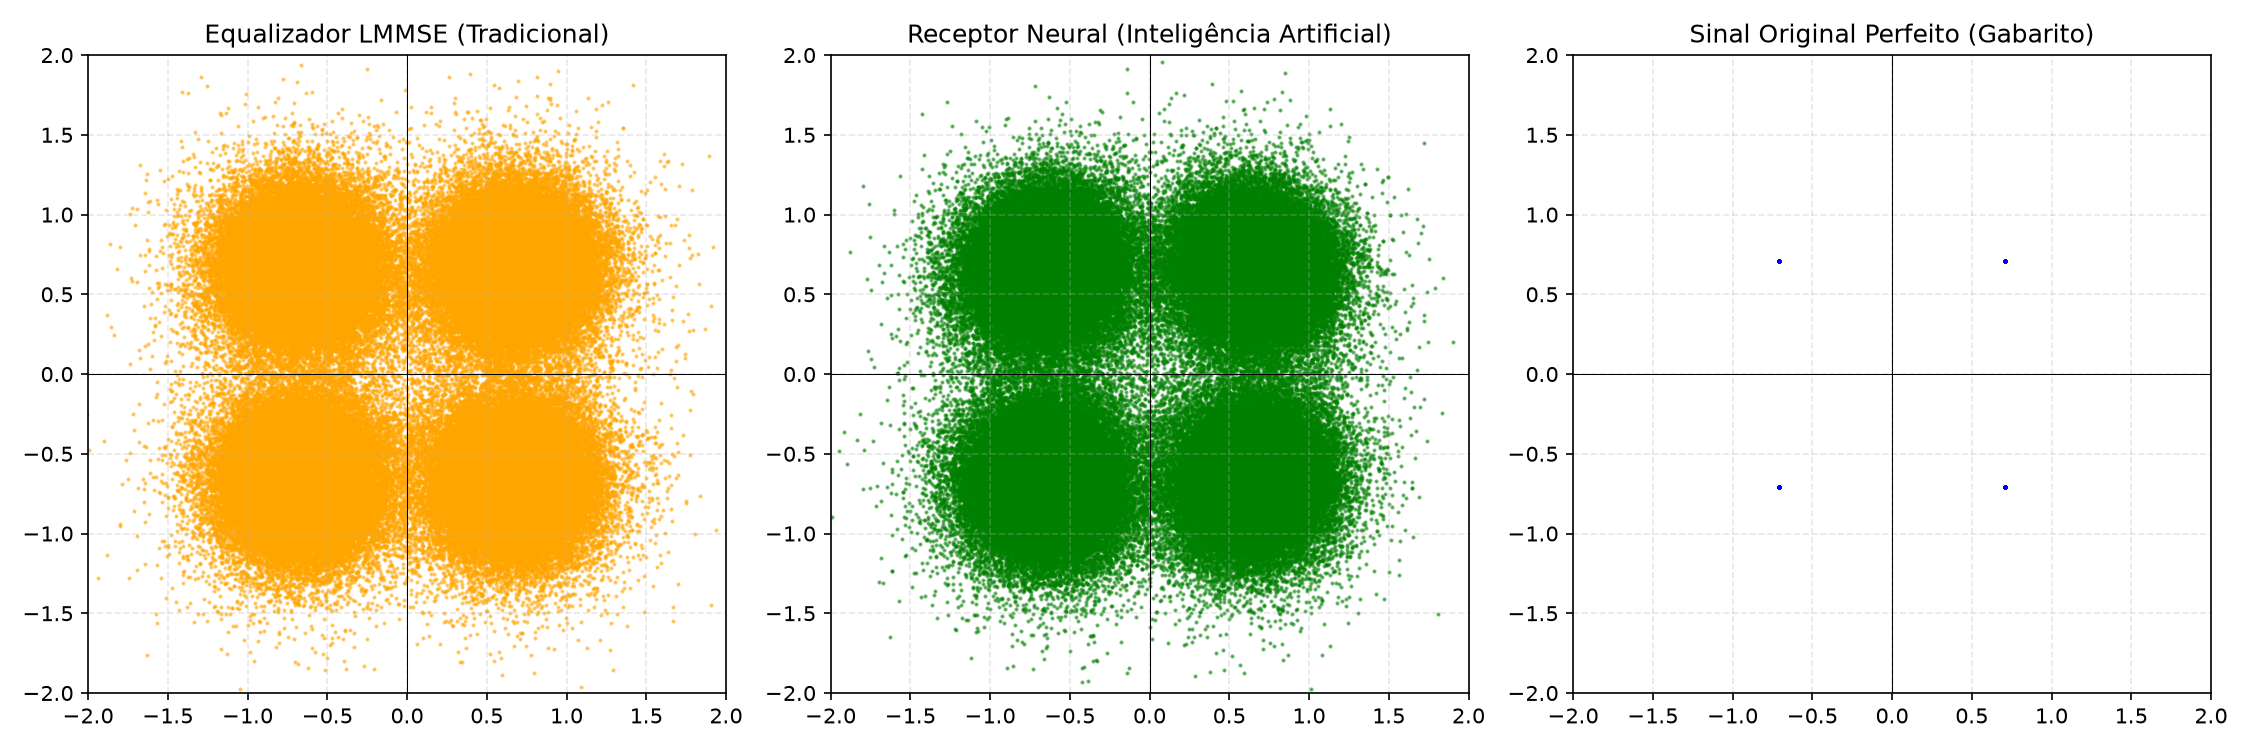
\includegraphics[width=\columnwidth]{figs/comparacao_neural_receiver.png}
    \caption{Dispersão em SNR Caótico (10 dB). A IA aprende empiricamente a mitigar os danos, enquanto a matriz LMMSE é sobrepujada por seu próprio ruído induzido.}
    \label{fig:comparacao_neural}
\end{figure}

\begin{figure}[htbp]
    \centering
    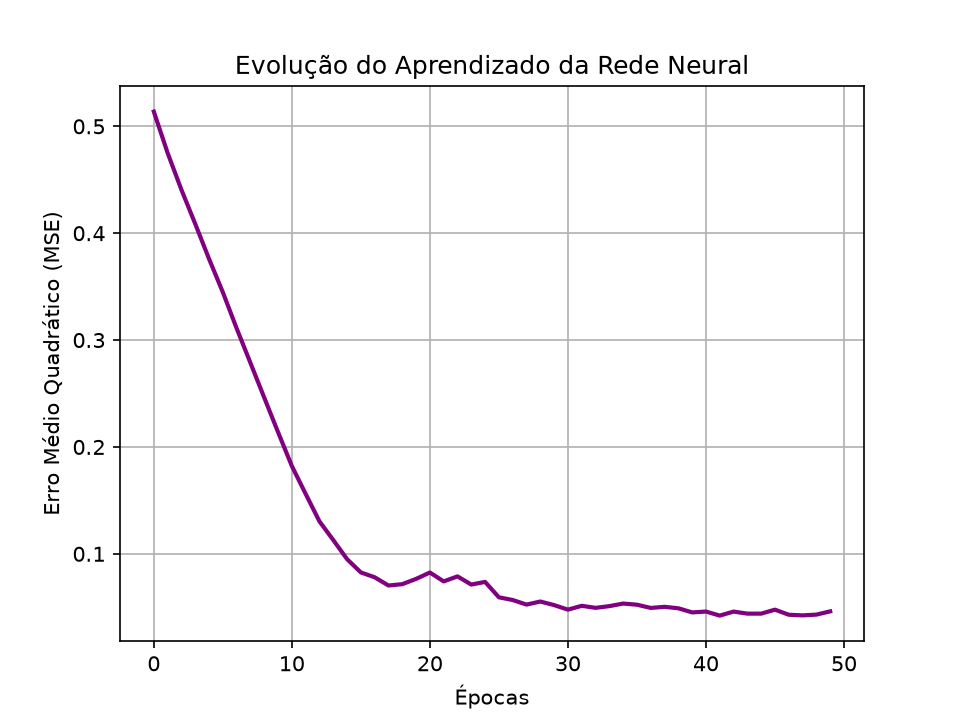
\includegraphics[width=\columnwidth]{figs/treinamento_neural.png}
    \caption{Convergência e queda do erro médio através de 50 épocas contínuas.}
    \label{fig:loss}
\end{figure}

\subsection{Alocação e Otimização Computacional}
O resultado acima justifica a pesquisa em Redes Neurais para o vindouro 6G não apenas pela precisão sob alta interferência. O gargalo computacional moderno reside na já citada inversão de matriz matemática do LMMSE com custo atrelado em $O(N^3)$, oneroso à eficiência de bateria das bases.
O Receptor Neural muda a arquitetura deste custo. O "estudo pesado" das matrizes é relegado à inferência supervisionada \textit{off-line} nas unidades computacionais centrais. Em operação na borda, as multiplicações em tensores \textit{forward-pass} das camadas neurais agem sob um patamar assintótico paralelizado de mera $O(N^2)$, tornando os dispositivos massivamente mais velozes e energicamente responsáveis \cite{hoydis2022}.

% ============================================
% 6. CONCLUSÃO
% ============================================
\section{Conclusão}

As simulações operadas permitiram solidificar os pilares matemáticos expostos na disciplina através de um framework industrial validado, expurgando problemas técnicos originários de implementações não padronizadas e atestando as curvas corretas de amortecimento do LMMSE em canais de alto desvanecimento, como dita a teoria. 

Superando o objetivo primário de replicação analítica estrita, propôs-se uma extrapolação baseada na moderna tecnologia habilitadora de \textit{Differentiable Communications}. Provou-se que Receptores Neurais operam com clareza superavitária sob ruídos ríspidos quando comparados ao limite clássico, além da arquitetura reverter o oneroso encargo elétrico-computacional de inversão matrizes $O(N^3)$ da borda em direções modulares, o que, consequentemente, impulsiona este tema como foco central para simulações acadêmicas do \textit{Massive MIMO}.

% ============================================
% REFERÊNCIAS
% ============================================
\begin{thebibliography}{00}

\bibitem{hoydis2022}
J.~Hoydis, S.~Cammerer, F.~Ait~Aoudia, A.~Vem, N.~Binder, G.~Marcus e A.~Keller, ``Sionna: An Open-Source Library for Next-Generation Physical Layer Research,'' \textit{arXiv preprint arXiv:2203.11854}, 2022.

\bibitem{sionna_tutorial}
NVIDIA, ``Sionna Tutorial: MIMO OFDM Transmissions over CDL,'' [Online]. Disponível em: \url{https://nvlabs.github.io/sionna/examples/MIMO_OFDM_Transmissions_over_CDL.html}. Acesso em: 25 jun. 2026.

\bibitem{proakis2008}
J.~G.~Proakis e M.~Salehi, \textit{Digital Communications}, 5ª~ed. Nova York, EUA: McGraw-Hill, 2008.

\bibitem{goldsmith2005}
A.~Goldsmith, \textit{Wireless Communications}. Cambridge, Reino Unido: Cambridge University Press, 2005.

\bibitem{vanDeBeek1995}
J.-J.~van~de~Beek, O.~Edfors, M.~Sandell, S.~K.~Wilson e P.~O.~Börjesson, ``On channel estimation in OFDM systems,'' in \textit{Proc. IEEE 45th Vehicular Technology Conference (VTC)}, 1995, pp.~815--819.

\bibitem{cammerer2023}
S.~Cammerer, F.~Ait~Aoudia, J.~Hoydis, A.~Vem, N.~Binder e A.~Keller, ``Trainable Communication Systems: Concepts and Prototype,'' \textit{IEEE Transactions on Communications}, vol.~71, no.~12, pp.~7328--7342, dez. 2023.

\bibitem{3gpp38211}
3GPP, ``NR; Physical channels and modulation,'' \textit{3rd Generation Partnership Project}, TS~38.211, 2023.

\bibitem{3gpp38901}
3GPP, ``Study on channel model for frequencies from 0.5 to 100~GHz,'' \textit{3rd Generation Partnership Project}, TR~38.901, v17.0.0, 2022.

\end{thebibliography}

\end{document}
